\documentclass[final]{beamer}
\usetheme{NTH}
\usepackage[orientation=portrait,size=a1,scale=1.4,debug]{beamerposter}
\usepackage[absolute,overlay]{textpos}
\usepackage{graphicx}
\usepackage{subfig}
\usepackage{multicol}
\usepackage{siunitx}
\setlength{\TPHorizModule}{1cm}
\setlength{\TPVertModule}{1cm}

\title{ Computational modelling of cell-cell transport via plasmodesmata }
\author{Nathan Hughes (hughesn@nbi.ac.uk)}
\footer{
  Email: \url{hughesn@nbi.ac.uk} |
  Twitter:
  \url{NathanHughes__}}
\date{\today}

\begin{document}
\begin{frame}{}

  \begin{textblock}{28}(1,4.5)

    \begin{block}{Plasmodesmata, what are they and why are they important?}

A key feature of multicellularity is the transfer of information
between cells for mutual benefit. The cell wall, a defining feature of
plant cells, separates cells and prevents molecules from being
freely transported from one cell to another. As a result, plants have evolved
microscopic channels known as plasmodesmata (PD) which span the cell
wall and connect the symplast of multiple cells \cite{chevalPlasmodesmalRegulationPlant2018}

\vspace{1cm}

During pathogen attack, PD have been show to close in order
to reduce intercellular flux. It is believed this is a defence
mechanism to help limit the spread of disease, thus understanding how
intercellular communications are influenced by changes to PD is vital
for further understanding defence responses in plants.

      \begin{figure}[!ht]
        \centering
        \subfloat[\label{subfig-1:plasdmodemsata}]{%
          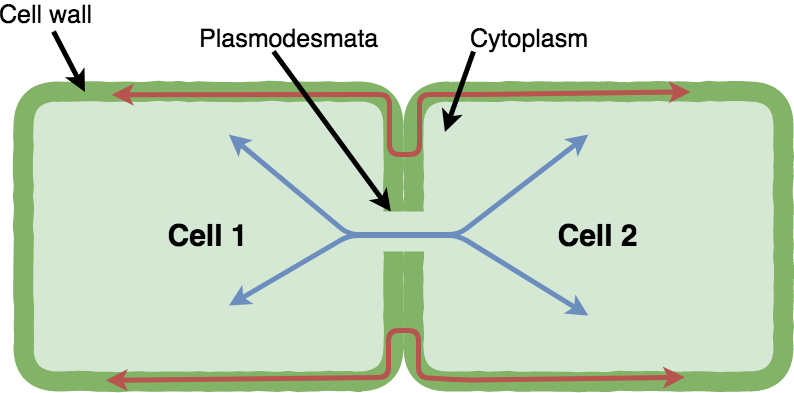
\includegraphics[width=0.75\columnwidth]{./figures/sympast+apoplast.png}
        }
        \\
        \subfloat[\label{subfig-2:plasdmodemsata}]{%
          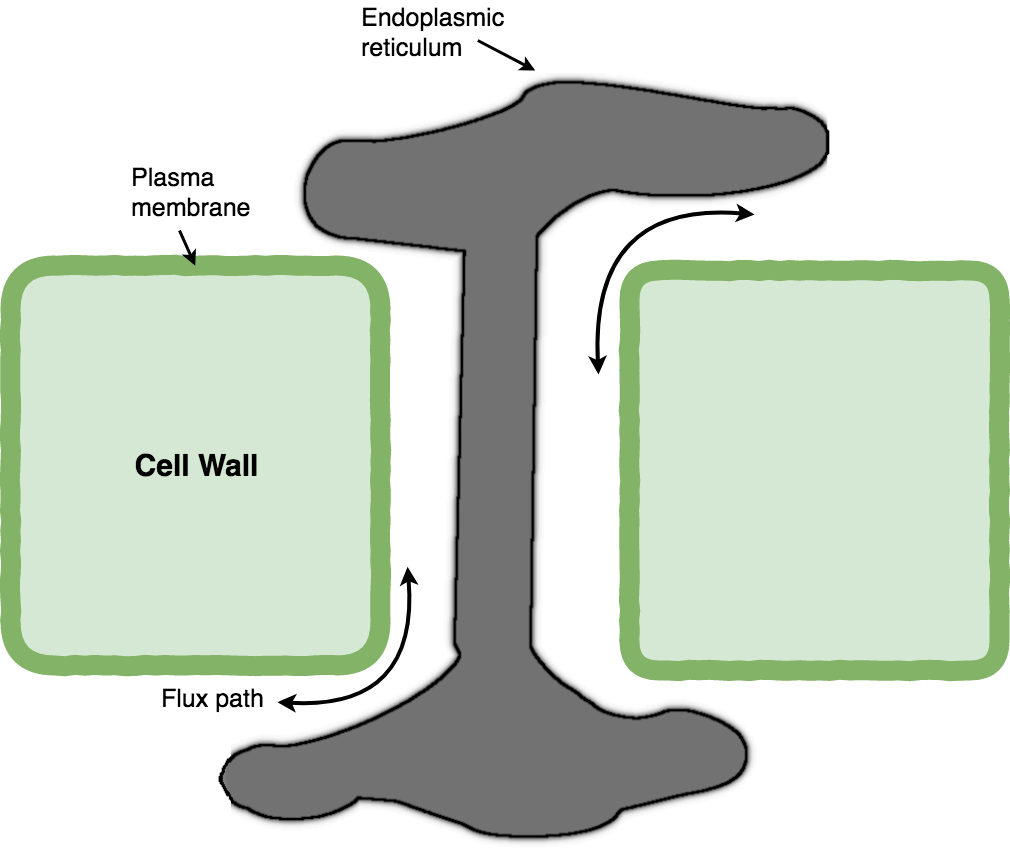
\includegraphics[width=0.45\columnwidth]{./figures/desmotubule.png}
        }
        \hfill
        \subfloat[\label{subfig-3:plasdmodemsata}]{%
          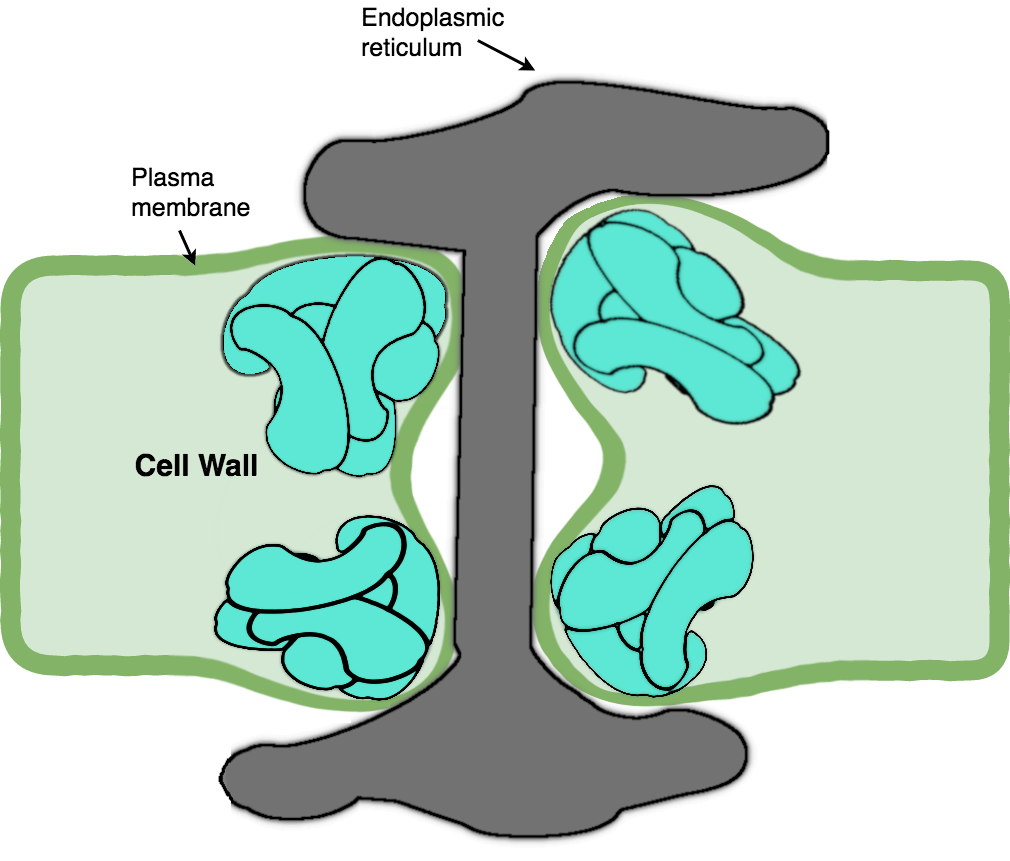
\includegraphics[width=0.45\columnwidth]{./figures/callose.png}
        }

        \caption[pd]{Plant cells are connected via plasmodesmata
          channels which span the cell wall of neighbouring cells,
          this allows for the diffusion of small molecules from
          cell to cell, (\textbf{a}). Plasmodesmata can
          modulate between open and closed via the deposition of callose in
          the cell wall, near plasmodesmata (\textbf{b-c})}
        \label{fig:pd}
      \end{figure}

    \end{block}

    \begin{block}{Modelling diffusion through the cell wall}

      To study the effects of the cell wall on intercellular diffusion
      we built a simple 1-D model of cells. With this model we
      simulated the diffusion of a molecule which at time 0 had a high
      concentration in a centre cell and absent from all other
      cells. Firstly, we tested this model with a cell wall which had
      no effect on diffusion and found, as expected, a typical
      diffusion curve.

      \vspace{1cm}

      Interestingly, we found that by reducing diffusion at the cell
      wall the concentration of the simulated molecule would quickly
      become uniform within each cell, but change drastically at the
      cell wall barriers. From these results, as well as Sobol
      sensitivity analysis on model parameters, highlight that the key
      determinant in intercellular diffusion is the permeability of
      the cell wall, which is ultimately a combination of PD density
      and aperture.

      % \textbf{a} Representation of the symplastic diffusion model in
      % 1D. (\textbf{b} and \textbf{c}) Symplastic concentrations of a diffusible
      % signalling molecule for different values of cell wall
      % permeability, $q$, that determine the flux through plasmodesmata
      % for a given concentration gradient. The consequences of high
      % permeability are shown in \textbf{b} and of low permeability in
      % \textbf{c}. This shows that cell wall permeability is a key parameter
      % for cell to cell communication.

      \begin{figure}[!ht]
        \centering
        \subfloat[\label{subfig-1:waterfall}]{%
          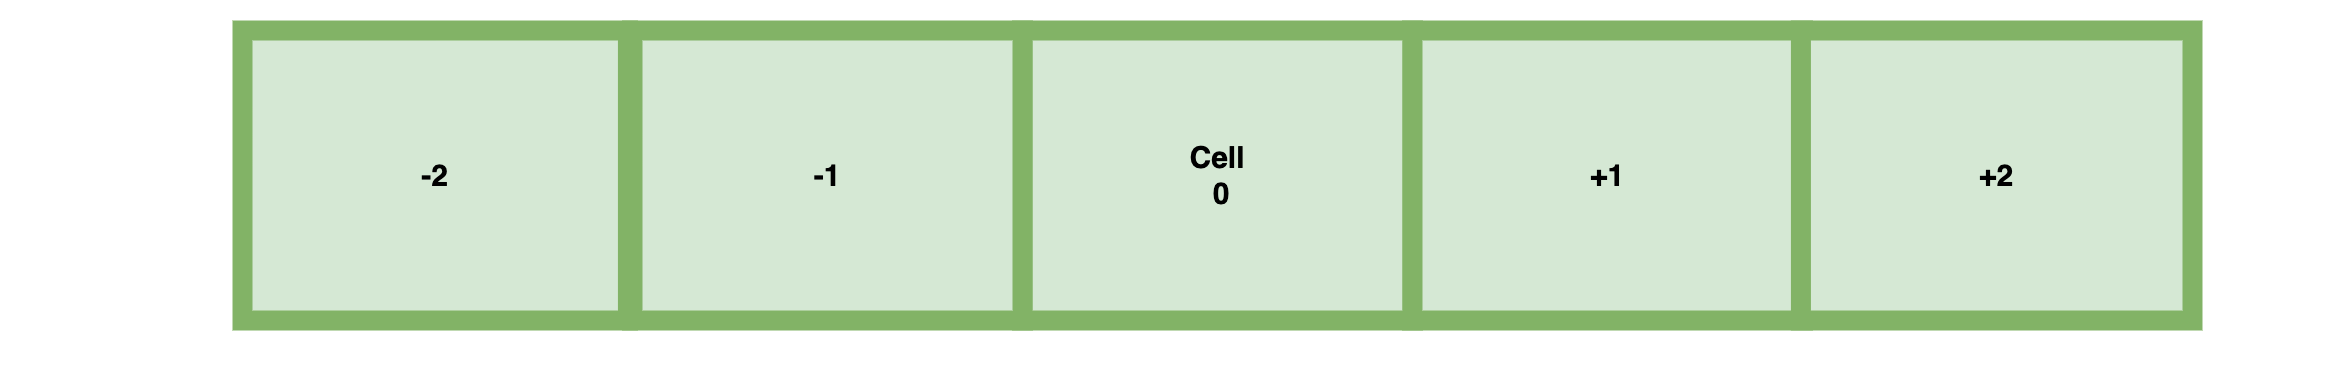
\includegraphics[width=0.975\columnwidth]{./figures/wf1.png}
        }
        \\
        \subfloat[\label{subfig-2:waterfall}]{%
          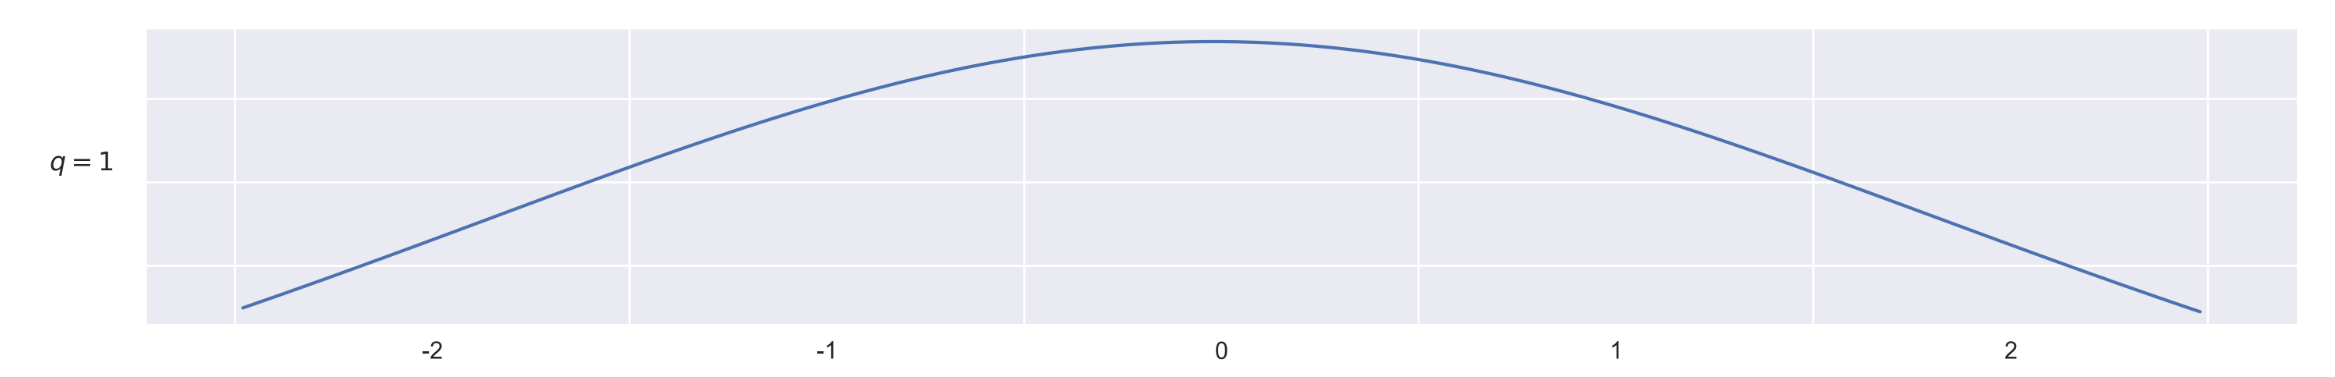
\includegraphics[width=0.975\columnwidth]{./figures/wf2.png}
        }
        \\
        \subfloat[\label{subfig-3:waterfall}]{%
          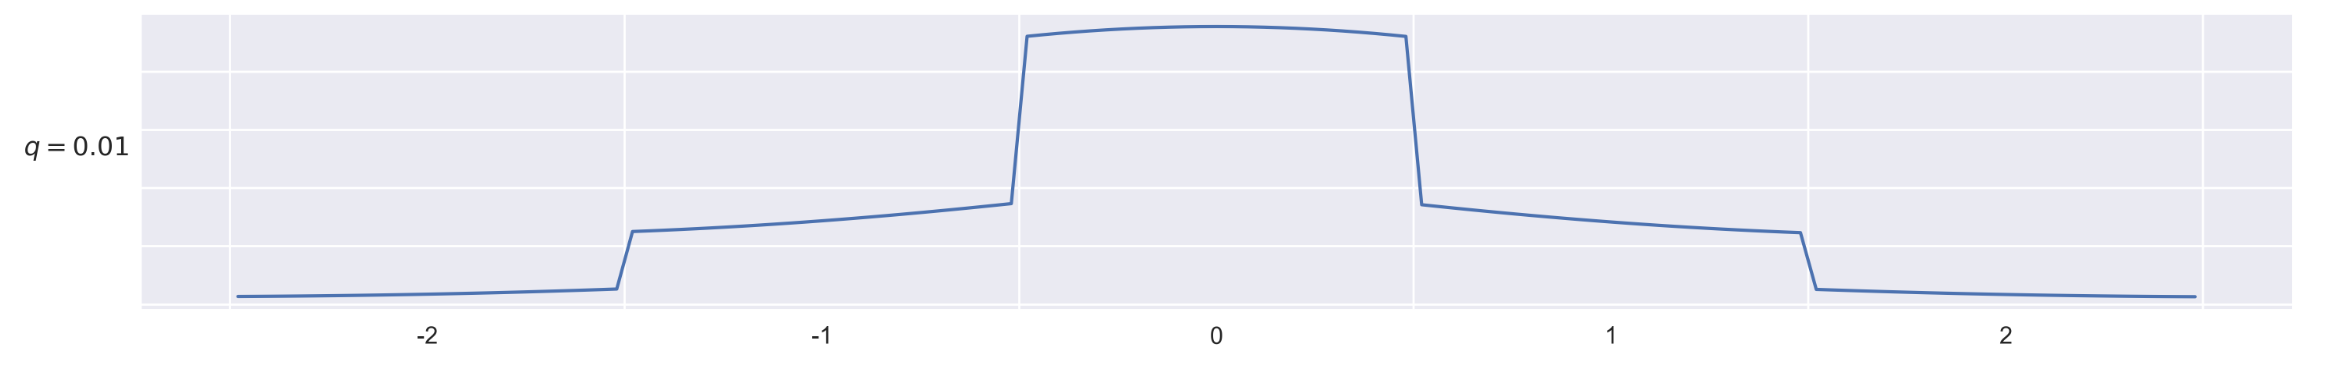
\includegraphics[width=0.975\columnwidth]{./figures/wf3.png}
        }

        \caption[1D symplastic diffusion model]{Pictorial
          representation of 1D symplastic diffusion model
          (\textbf{a}). Cell wall permeability is the key determinant
          in cell to cell diffusion (\textbf{b-c}) }
        \label{fig:diff}
      \end{figure}


    \end{block}



  \end{textblock}

  \begin{textblock}{28}(30.5,4.5)

    \begin{block}{Cell to cell signalling as a narrow escape problem}

      \begin{multicols}{2}

        In order to further study how molecules move from cell to cell
        we evaluated the so-called Narrow Escape Problem for use in
        plant cell models \cite{holcmanEscapeSmallOpening2004}.

        \vspace{1cm}

        The narrow escape problem considers a particle within a
        container, under Brownian motion the particle moves within the
        container until it reaches a specified opening on the surface
        through which it may escape.


        \vspace{1cm}

        A number of solutions have been previously derived for this
        problem which are able to give a mean escape time
        estimation. Using our own simulations we verified these
        solutions and found them to be well suited and applicable for
        plant-cell parameters.

        \columnbreak


      \begin{figure}[!ht]
        \centering
          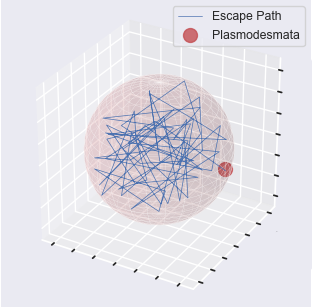
\includegraphics[width=0.9\columnwidth]{./figures/escape_example.png}
        \caption[Narrow Escape Example]{An example of the narrow
          escape problem, solved with a random walk simulation. A
          particle takes a path (shown in blue) within a cell,
          eventually it passes through a plasmodesmatal pore (red dot)
          allowing it to move to a neighbouring cell}
        \label{fig:nepfig}
      \end{figure}
    \end{multicols}
    \end{block}

    \begin{block}{Evaluating the narrow escape problem for plant cells}

      The narrow escape solutions were produced for spheres, plant
      cells are much more complex in shape. Thus, we simulated a range
      of ellipsoid shapes to find the limits of the narrow escape solutions.

      \vspace{1cm}

      We found that the narrow escape solutions could capture the
      mean escape time for asymmetric shapes which had a sphericity of
      $>0.75$. Using 3D imaging data for both root and leaf tissue we
      found that the mean sphericity of these cell types are within
      the range we propose that the narrow escape solution is
      applicable.

      \begin{figure}[!ht]
        \centering
        \subfloat[\label{subfig-1:waterfall}]{%
          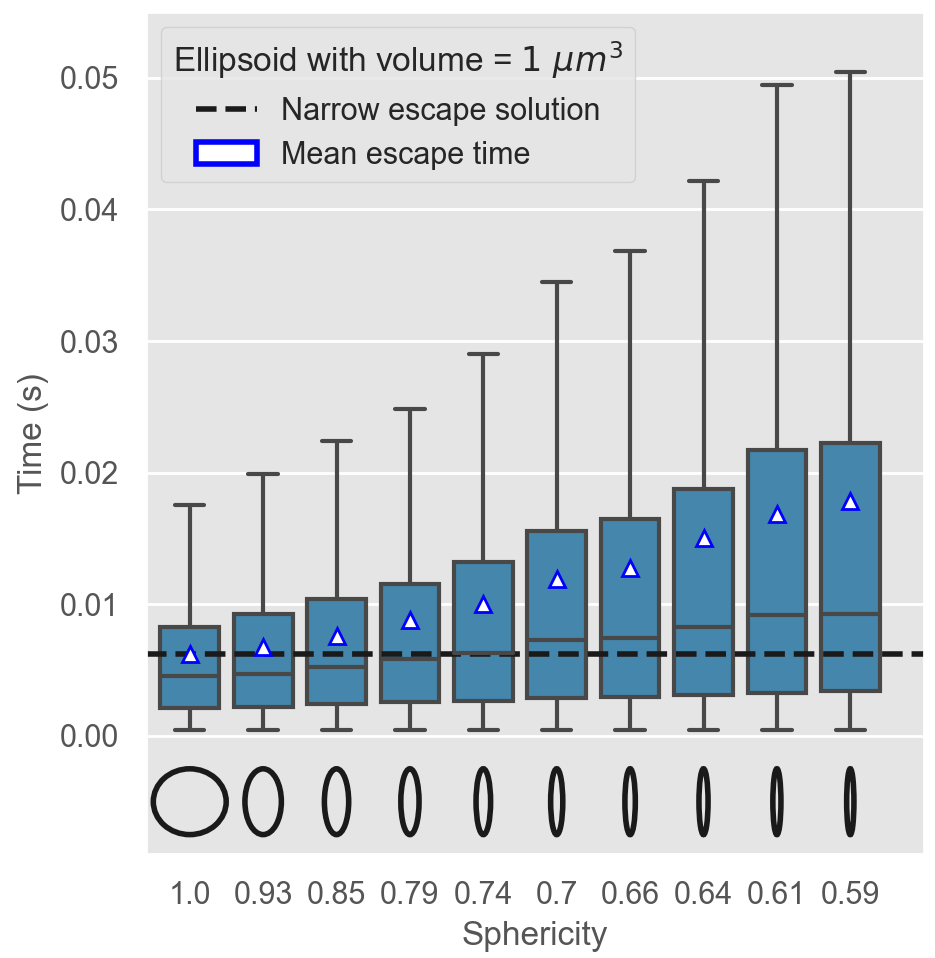
\includegraphics[width=0.42\columnwidth]{./figures/spheroid_m.png}
        }
        \subfloat[\label{subfig-2:waterfall}]{%
          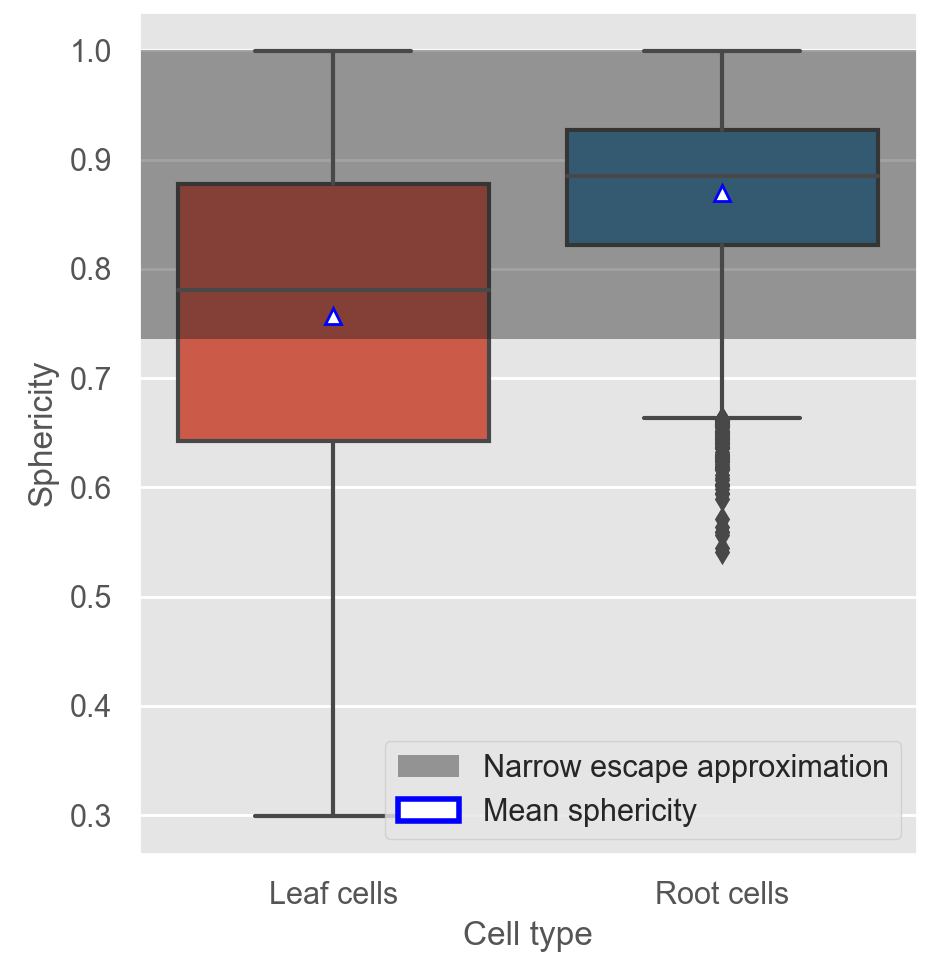
\includegraphics[width=0.42\columnwidth]{./figures/spheroid_b.png}
        }

        \caption[NarrowEp]{Testing the narrow escape solutions for a
          range of elongated ellipsoids (\textbf{a}). Evaluating the
          sphericity of 3D shows that the narrow escape solutions can
          approximate the escape time for realistic cell shapes \textbf{(b)}}
        \label{fig:nep}
      \end{figure}


    \end{block}


    \begin{block}{Future work}

      Currently, we are incorporating the narrow escape
      solutions into other models we have been using. Primarily
      network based models which will allow for tissue scale
      simulations of various pathogen themed conditions.

      \vspace{1cm}

      With these future models we will focus on features such as
      plasmodesmata density and aperture. We will then analyse how
      these change and alter under simulated pathogen stresses. From
      these we will produce hypotheses on how plant cells communicate
      while under pathogen attack.

    \end{block}



    \begin{block}{Acknowledgements}
      Thank you for the vital help and support from the following.

      \begin{multicols}{3}

        \begin{itemize}
        \item{Prof. Richard Morris}
        \item{Dr. Christine Faulkner}

        \end{itemize}

        \columnbreak

        \begin{itemize}
        \item{Dr. Melissa Tomkins}
        \item{Morris \& Faulkner Groups}

        \end{itemize}

        \columnbreak

        \begin{itemize}
        \item{BBSRC}
        \item{NRPDTP}
        \end{itemize}

      \end{multicols}

    \end{block}

    \begin{block}{References}
      \bibliography{poster}
      \bibliographystyle{unsrt}
    \end{block}


  \end{textblock}

\end{frame}
\end{document}

%%% Local Variables:
%%% mode: latex
%%% TeX-master: t
%%% End:
